\documentclass[12pt,onecolumn]{article}
\usepackage{listings}
\usepackage{float}
\usepackage{mathtools}
\usepackage[russian]{babel}
\everymath{\displaystyle}
\usepackage{placeins}
\usepackage[table,xcdraw]{xcolor}
\usepackage{geometry}
\geometry{
  a4paper,
  top=25mm, 
  right=15mm, 
  bottom=25mm, 
  left=15mm
}

\begin{document}
\setcounter{tocdepth}{4}
\begin{center}
    Санкт-Петербургский Национальный Исследовательский\\ 
    Университет ИТМО\\
    Мегафакультет Компьютерных Технологий и Управления\\
    Факультет Программной Инженерии и Компьютерной Техники \\
    
\includegraphics[scale=0.3]{itm.jpg} % нужно закинуть картинку логтипа в папку с отчетом
\end{center}
\vspace{1cm}


\begin{center}
    \large \textbf{Вариант №666666}\\
    \textbf{Лабораторная работа №2}\\
    по дисциплине\\
    \textbf{Программирование}
\end{center}

\vspace{2cm}

\begin{flushright}
  Выполнил Студент  группы P3116\\
  \textbf{Алексей Лапин}\\
  Преподаватель: \\
  \textbf{Сорокин Роман Борисович}\\
\end{flushright}

\vspace{10cm}
\begin{center}
    г. Санкт-Петербург\\
    2021г.
\end{center}
\newpage
\tableofcontents
\newpage
\section{Текст задания}
На основе базового класса Pokemon написать свои классы для заданных видов покемонов. Каждый вид покемона должен иметь один или два типа и стандартные базовые характеристики:
\begin{itemize}
    \item очки здоровья (HP)
    \item атака (attack)
    \item защита (defense)
    \item специальная атака (special attack)
    \item специальная защита (special defense)
    \item скорость (speed)
\end{itemize}
Классы покемонов должны наследоваться в соответствии с цепочкой эволюции покемонов. На основе базовых классов PhysicalMove, SpecialMove и StatusMove реализовать свои классы для заданных видов атак.

Атака должна иметь стандартные тип, силу (power) и точность (accuracy). Должны быть реализованы стандартные эффекты атаки. Назначить каждому виду покемонов атаки в соответствии с вариантом. Уровень покемона выбирается минимально необходимым для всех реализованных атак.

Используя класс симуляции боя Battle, создать 2 команды покемонов (каждый покемон должен иметь имя) и запустить бой.

Базовые классы и симулятор сражения находятся в jar-архиве (обновлен 9.10.2018, исправлен баг с добавлением атак и кодировкой). Документация в формате javadoc - здесь.

Информацию о покемонах, цепочках эволюции и атаках можно найти на сайтах http://poke-universe.ru, http://pokemondb.net, http://veekun.com/dex/pokemon
\section{Покемоны}
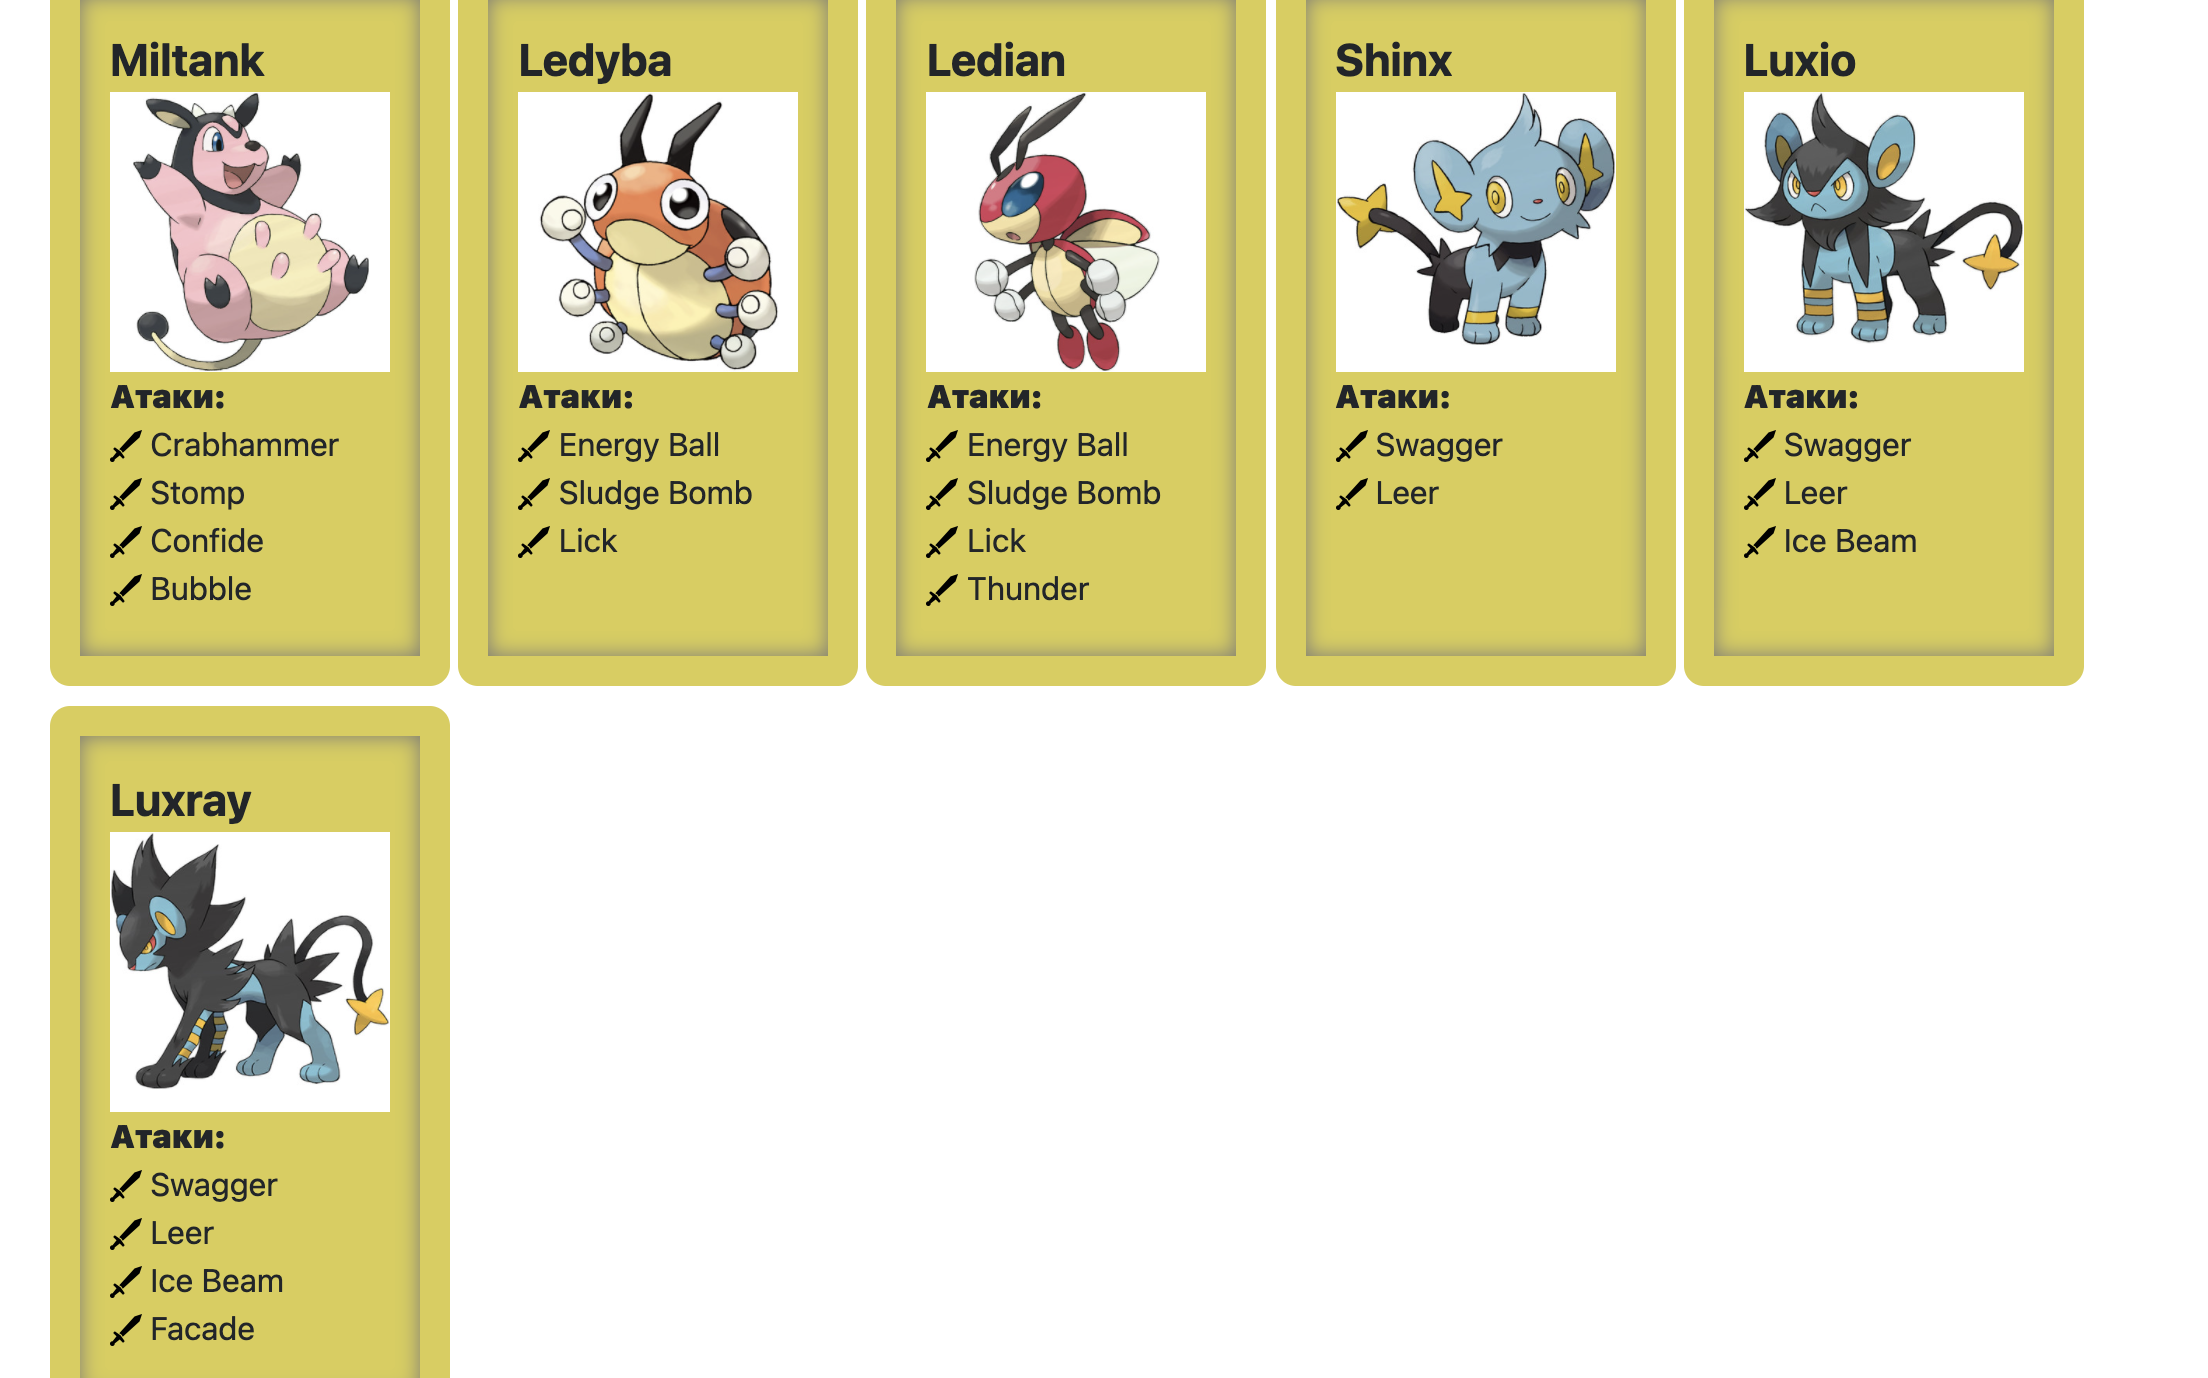
\includegraphics[scale=0.3]{pokemons.png}
\section{Диаграмма классов}
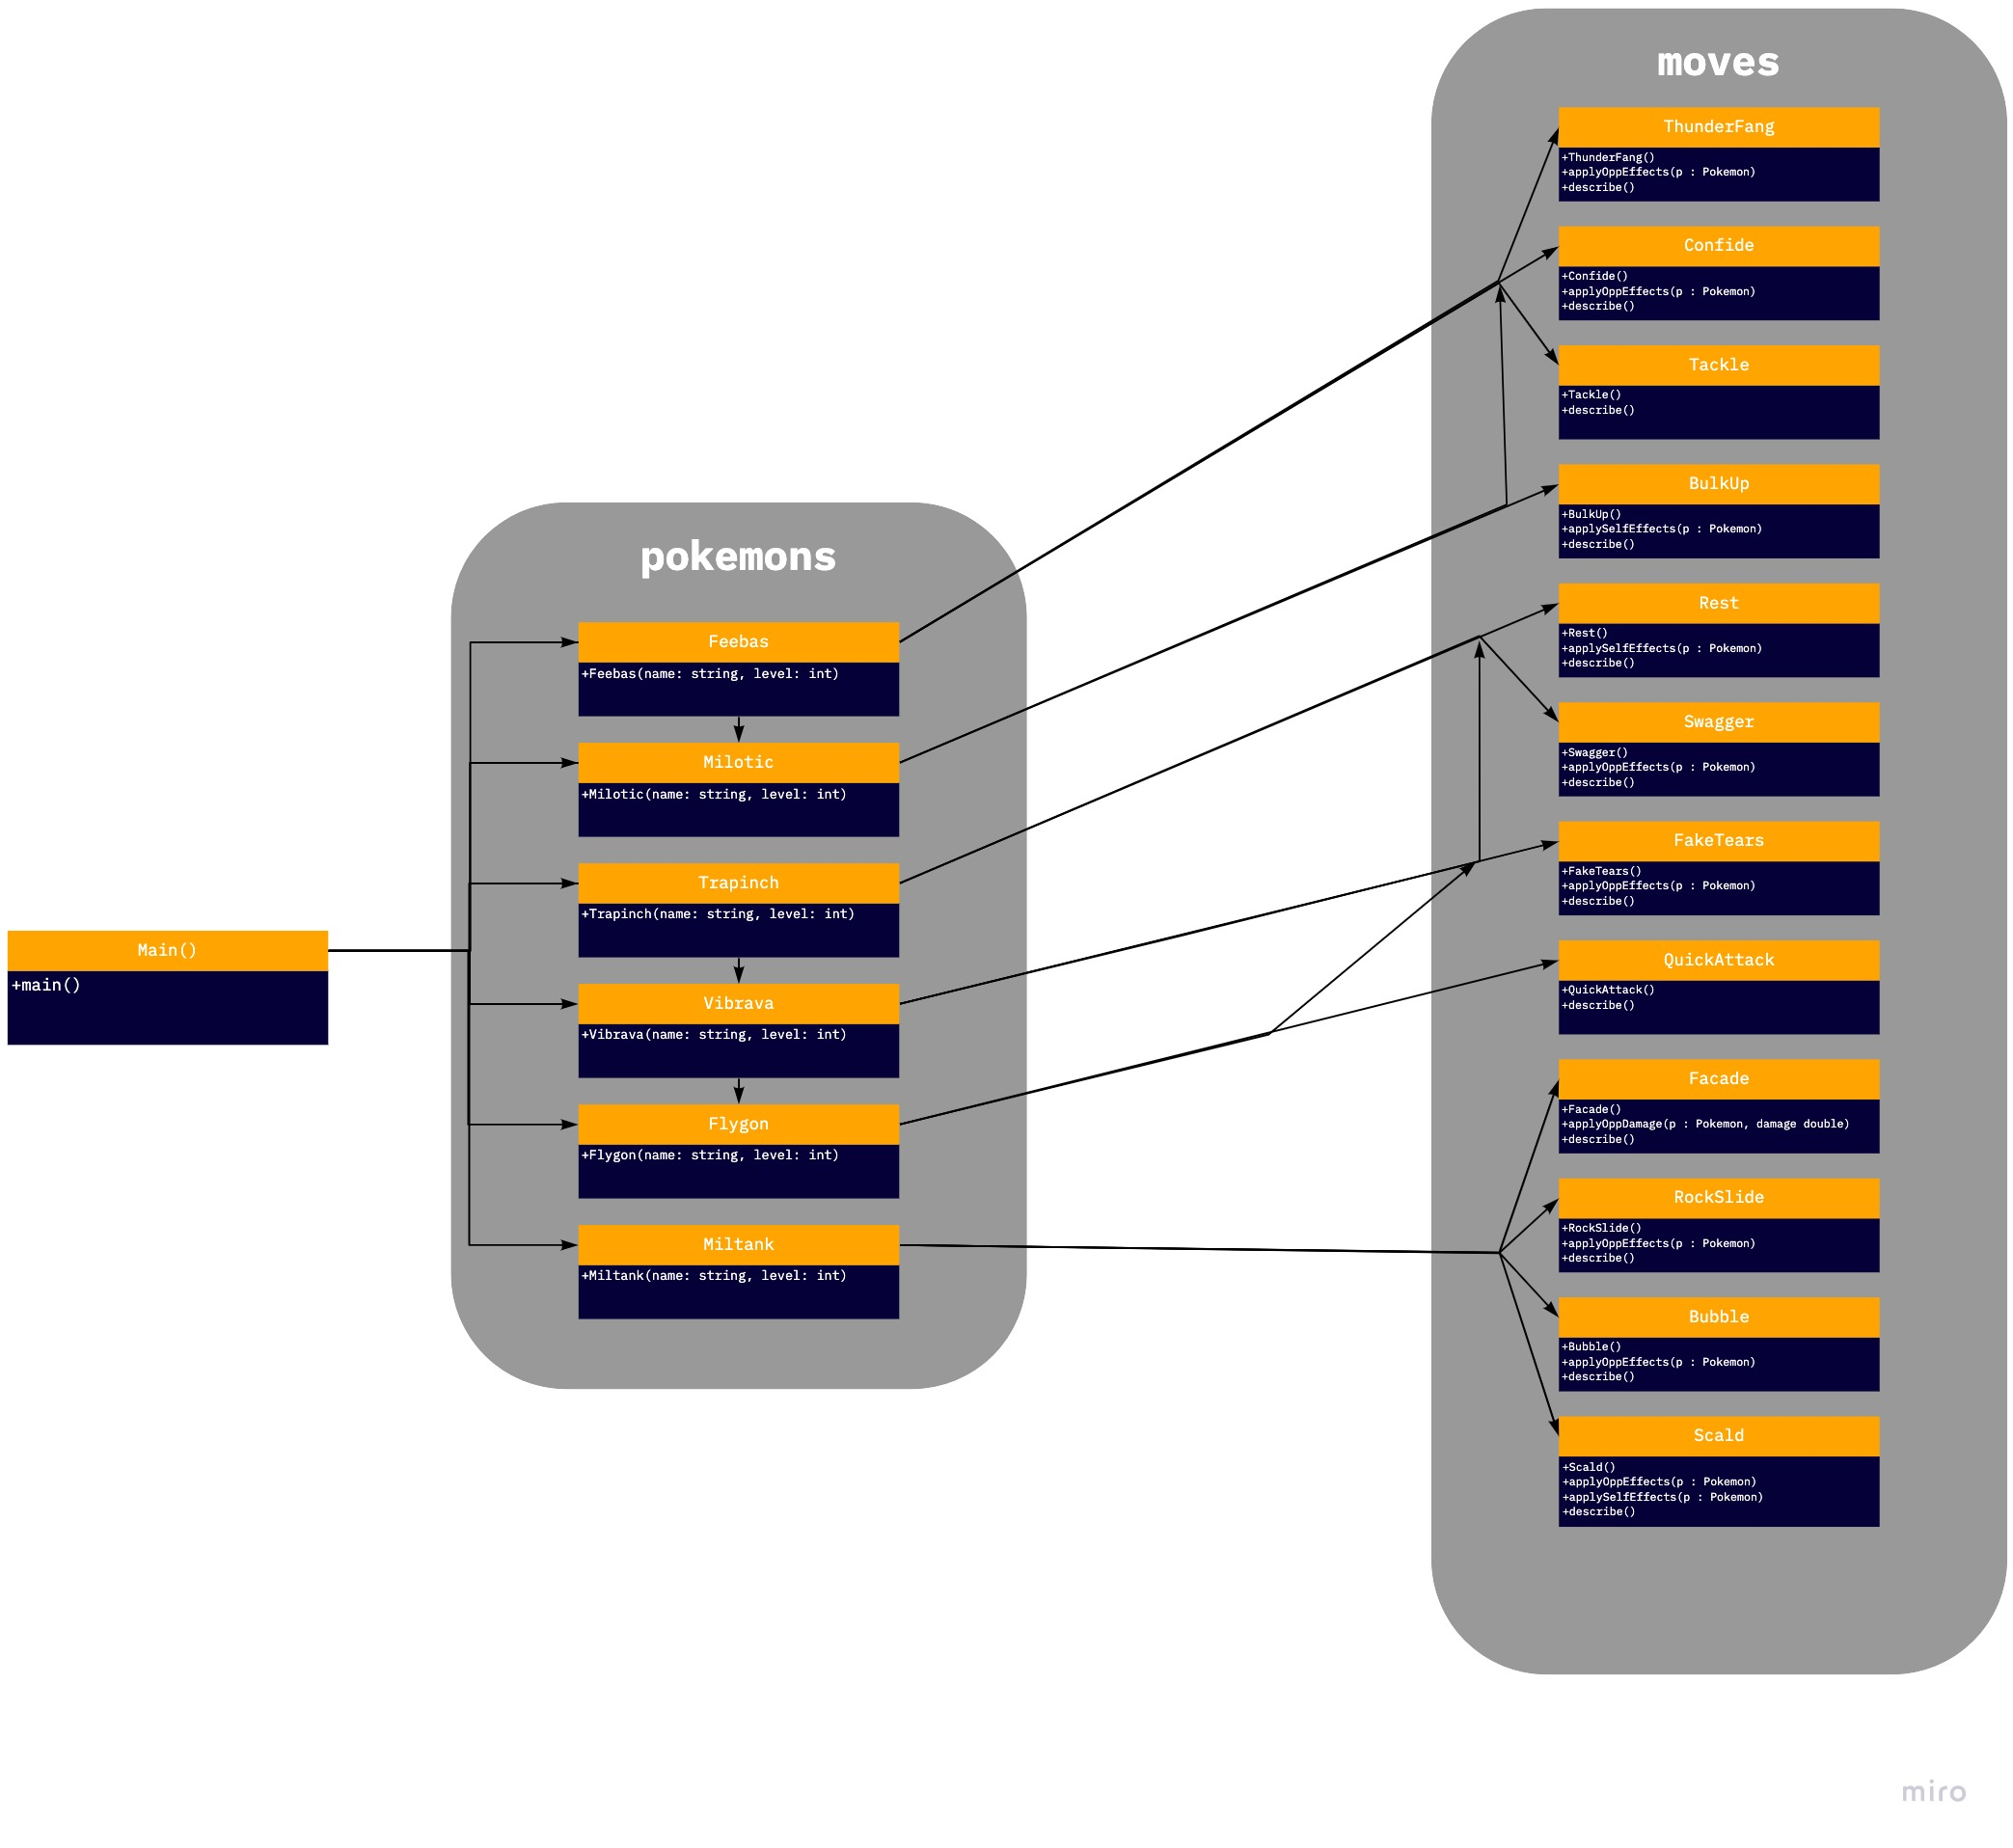
\includegraphics[scale=0.25]{UML.jpg}
\section{Исходный код программы}
\lstloadlanguages{Java}
\definecolor{mygray}{RGB}{120,120,120}
\lstset{extendedchars =/true,
breaklines=true,
basicstyle=\ttfamily\fontsize{9pt}{9pt}\selectfont,
commentstyle=\color{mygray},
keywordstyle=\color{blue}}
Main.java
\lstinputlisting[language=Java,numbers=left]{src/Main.java}
Pokemons\\
Feebas.java
\lstinputlisting[language=Java,numbers=left]{src/pokemons/Feebas.java}
Flygon.java
\lstinputlisting[language=Java,numbers=left]{src/pokemons/Flygon.java}
Milotic.java
\lstinputlisting[language=Java,numbers=left]{src/pokemons/Milotic.java}
Miltank.java
\lstinputlisting[language=Java,numbers=left]{src/pokemons/Miltank.java}
Trapinch.java
\lstinputlisting[language=Java,numbers=left]{src/pokemons/Trapinch.java}
Vibrava.java
\lstinputlisting[language=Java,numbers=left]{src/pokemons/Vibrava.java}
Moves\\
Bubble.java
\lstinputlisting[language=Java,numbers=left]{src/moves/Bubble.java}
BulkUp.java
\lstinputlisting[language=Java,numbers=left]{src/moves/BulkUp.java}
Confide.java
\lstinputlisting[language=Java,numbers=left]{src/moves/Confide.java}
Facade.java
\lstinputlisting[language=Java,numbers=left]{src/moves/Facade.java}
FakeTears.java
\lstinputlisting[language=Java,numbers=left]{src/moves/FakeTears.java}
QuickAttack.java
\lstinputlisting[language=Java,numbers=left]{src/moves/QuickAttack.java}
Rest.java
\lstinputlisting[language=Java,numbers=left]{src/moves/Rest.java}
RockSlide.java
\lstinputlisting[language=Java,numbers=left]{src/moves/RockSlide.java}
Scald.java
\lstinputlisting[language=Java,numbers=left]{src/moves/Scald.java}
Swagger.java
\lstinputlisting[language=Java,numbers=left]{src/moves/Swagger.java}
Tackle.java
\lstinputlisting[language=Java,numbers=left]{src/moves/Tackle.java}
ThunderFang.java
\lstinputlisting[language=Java,numbers=left]{src/moves/ThunderFang.java}
\section{Результат выполнения:}
\tiny{
Feebas Дирихле из команды фиолетовых вступает в бой!\\
Miltank Вейерштрасс из команды зеленых вступает в бой!\\
Miltank Вейерштрасс using Scald. \\
Feebas Дирихле теряет 2 здоровья.\\
Feebas Дирихле воспламеняется\\
\hfill \break
Feebas Дирихле using Thunder Fang. \\
Miltank Вейерштрасс восстанавливает 1 здоровья.\\
\hfill \break
Feebas Дирихле using Tackle. \\
Miltank Вейерштрасс восстанавливает 1 здоровья.\\
\hfill \break
Miltank Вейерштрасс using Bubble. \\
Feebas Дирихле теряет 1 здоровья.\\
\hfill \break
Feebas Дирихле using Tackle. \\
Miltank Вейерштрасс восстанавливает 1 здоровья.\\
\hfill \break
Miltank Вейерштрасс using Rock Slide. \\
Feebas Дирихле теряет 4 здоровья.\\
\hfill \break
Feebas Дирихле using Thunder Fang. \\
Miltank Вейерштрасс восстанавливает 1 здоровья.\\
\hfill \break
Miltank Вейерштрасс using Scald. \\
Feebas Дирихле теряет 3 здоровья.\\
\hfill \break
Feebas Дирихле using Thunder Fang. \\
Miltank Вейерштрасс восстанавливает 1 здоровья.\\
Miltank Вейерштрасс парализован\\
\hfill \break
Miltank Вейерштрасс using Rock Slide. \\
Критический удар!\\
Feebas Дирихле теряет 11 здоровья.\\
Feebas Дирихле теряет сознание.\\
Flygon Коши из команды фиолетовых вступает в бой!\\
Miltank Вейерштрасс using Facade. \\
Критический удар!\\
Flygon Коши теряет 11 здоровья.\\
\hfill \break
Flygon Коши промахивается\\
\hfill \break
Flygon Коши using Quick Attack. \\
Miltank Вейерштрасс теряет 3 здоровья.\\
\hfill \break
Miltank Вейерштрасс using Scald. \\
Критический удар!\\
Flygon Коши теряет 13 здоровья.\\
Flygon Коши воспламеняется\\
Flygon Коши теряет сознание.\\
Milotic Лагранж из команды фиолетовых вступает в бой!\\
Miltank Вейерштрасс using Rock Slide. \\
Критический удар!\\
Milotic Лагранж теряет 9 здоровья.\\
\hfill \break
Milotic Лагранж using Thunder Fang. \\
Miltank Вейерштрасс теряет 4 здоровья.\\
\hfill \break
Miltank Вейерштрасс using Facade. \\
Критический удар!\\
Milotic Лагранж теряет 12 здоровья.\\
Milotic Лагранж теряет сознание.\\
В команде фиолетовых не осталось покемонов.\\
Команда зеленых побеждает в этом бою!\\
}
\section{Вывод}
\normalsize
В процессе выполнения этой лабораторной работы я познакомился с основными принципами объектно-ориентированное программирование в языке Java.
Научился работать с методами, классами, модификаторами доступа и сторонними библиотеками.
\end{document}